\vspace{-5px}\section{Hogwild! Inference}\label{sect:method}\vspace{-5px}

Our main intuition is that modern LLMs do not need a pre-defined framework for inference-time parallelism: they can organize it by themselves. 
To test this hypothesis, we design a parallel inference protocol where multiple LLM instances can collaborate as flexibly as possible. Instead of assigning each ``worker'' to a specific role or sub-task, we run them in parallel and prompt them to come up with their own means of working together. This approach has two key components: how to run multiple inference threads from the same Key-Value memory, and how to prompt LLM ``workers'' to collaborate over said memory. To that end, we organize this section as follows: we first outline how to perform LLM inference with a shared cache in Section~\ref{sect:method_basic_idea}. Then, in Section~\ref{sect:method_cache_layouts} we describe several possible memory layouts and their implications.
Finally, in Section~\ref{sect:method_prompting}, we describe our strategy for prompting LLMs to collaborate.

\vspace{-5px}\subsection{Concurrent Attention with Shared Key-Value Cache}\label{sect:method_basic_idea}\vspace{-5px}

The core ingredient of Hogwild!\! Inference is a shared Key-Value memory (KV cache) accessible to all workers. The cache consists of several blocks that can be reused between workers, implementing a \textbf{concurrent version of the attention mechanism}~\citep{bahdanau2014neural, vaswani2017attention}. 

Let us first consider the simplest case of Hogwild! Inference with two workers and three cache blocks, as depicted in Figure~\ref{fig:teaser}. The first block contains the prompt, and the other two blocks contain the ``thoughts'' (tokens generated) by workers A and B respectively (denoted Alice and Bob in the Figure).
As workers generate new tokens, they access each other's attention caches as though these were their own previously generated tokens. In Figure~\ref{fig:teaser}, ``Alice'' sees the common prompt, then ``Bob's'' token representations, then her own. In turn, Bob sees the same common prompt, then Alice's token KVs, and his own tokens after that.\footnote[3]{For clarity of exposition, we choose to anthropomorphize the pronouns for these two parallel agents.} 

This creates a discrepancy where the same Key-Value pairs appear on different positions for each worker. Furthermore, the relative distance between the same pair of tokens (e.g., first generated tokens from Alice and Bob, respectively) changes as new tokens are added. While it is possible to re-encode these tokens at their new position, it would cause computation overhead that scales cubically\footnote[4]{If $n$ agents generate one new token each, which is then re-encoded differently for each of these $n$ agents, that each have to attend to $O(n)$ additional tokens, then the total step complexity is $O(n^3)$.}.

Instead of re-encoding the new tokens for other workers, we attempt to reuse existing token representations between workers. However, since these tokens appear at different positions for each worker and step, we need to adjust for their positional embeddings.
Most modern LLMs use Rotary Position Embeddings (RoPE)~\citep{su2021roformer}, where each key and query is rotated to an angle proportional to its absolute position. Prior works have shown that RoPE embeddings can be manipulated through scaling~\citep{rope_scaling} slicing~\citep{streamingllm}, or pruning~\citep{zhang2023h2o}. One very useful property of RoPE embeddings is that they are invariant to parallel shifts in position: if both query and key are rotated by the same angle, the dot product between them will not change. 

In Hogwild!\! Inference, we rely on this property and rotate the entire KV blocks to their position during inference. As shown in Figure~\ref{fig:teaser} (right), the same cache blocks are arranged in different order for each worker, but the relative angle between the tokens within each block stays the same. In other words, the attention score between Alice's last token and her previous tokens does not change from this parallel shift, but she also gains access to Bob's tokens and vice versa.

When generating new tokens in this manner, we perform a forward pass on all workers in parallel, as though they were samples in the same batch.
When processing newly generated tokens, we insert their KV representations at the end of their respective cache blocks, then arrange these cache blocks for each worker. This way, both workers can immediately attend to each other's latest tokens even before they are fully processed by all model layers.
Since re-arranging the cache takes up memory for each worker, we materialize the rearranged Key-Value cache for one attention layer at a time, just-in-time for computation.
% We discuss the technical details further in Appendix~\ref{sect:appendix_implementation}.

\begin{figure}[t]
    \centering
    \vspace{-20px}
    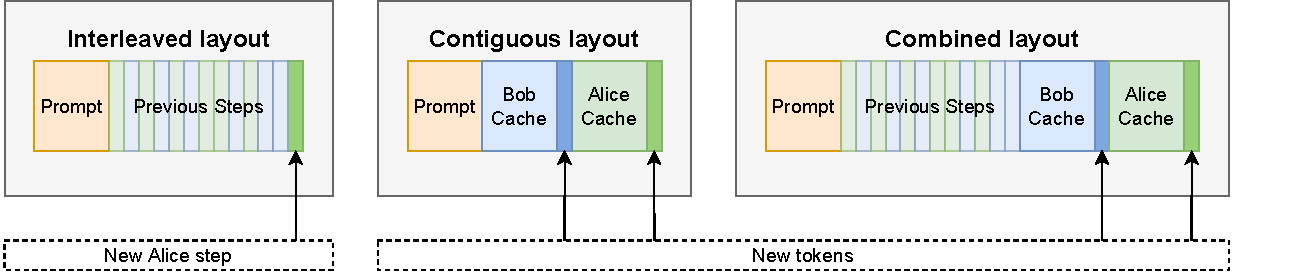
\includegraphics[width=1.045\linewidth,height=82px]{resources/figure2_fixed.pdf}
    \caption{Three cache layouts described in Section~\ref{sect:method_cache_layouts}: interleaved with step-wise synchrony (left), simple contiguous layout (middle) and combined with token-wise synchrony (right). All layouts are made from Alice point of view.}
    \label{fig:layouts}\vspace{-15px}
\end{figure}


\vspace{-5px}\subsection{Cache Layouts}\label{sect:method_cache_layouts}\vspace{-5px}

Now that we established that a cache can be split into blocks and rearranged on the fly, it is reasonable to ask how best to arrange those blocks. In this preliminary study, we consider three such arrangements, shown at Figure \ref{fig:layouts}.

\textbf{Contiguous layout (token-wise)} is the simplest possible layout
where each worker appends to their own sequence blob of tokens and sees other workers' token representations as past keys and values. This layout is inspired by collaborative text editors such as Google Docs or Overleaf.

As described earlier in Section~\ref{sect:method_basic_idea}, each worker arranges the other workers' thoughts in a different order. They see the common prompt cache first, then the caches of all \textit{other} workers (excluding themselves\footnote[5]{When extending this layout to more than 2 workers, each worker sees the key-value memories of everyone except themselves. For instance, given 3 workers A, B, and C, worker B will see a version of the cache that contains the prompt, outputs of workers A and C, and finally, B's own memory. Likewise, A sees B \& C, then A. }), then their own cache as immediate previous tokens. That way, each worker predicts the next token for their own cache.

\textbf{Interleaved layout (step-wise),} which can be seen as analogous to group chat services such as Slack or Discord. In this layout, workers generate tokens \textit{in private} until they finish a reasoning step\footnote[6]{We define a reasoning step as any amount of text that ends with a complete sentence, e.g. a dot or a question mark, and then a double newline (\texttt{"\textbackslash n\textbackslash n"}) in all our experiments, though it may vary by the model.}, then add it to a shared ``history''.
The history contains past reasoning steps of each LLM instance in the order of their completion. Whenever a worker completes a reasoning step, their KV cache entries are moved to the end of the shared history cache block with the proper rotation, then their local cache is reset their local cache for a new step.

In this setup, the workers only see each other's outputs in full steps, not after every token. However, they do not wait for each other to complete their steps. Instead, each worker keeps generating new tokens and occasionally receives additional key-value pairs inserted into its cache.

\textbf{Combined layout (token-wise)} is a mixture of the first two.
The LLM instances 
generate steps that are accumulated in a shared history, as in the interleaved layout. However, they do not generate these steps in private, but can instantly see each other's current progress, as in the contiguous layout.

We can view the first two layouts as ablated versions of this combined one: the contiguous layout lacks the shared history, and the interleaved layout lacks immediate synchronization. We compare these three layouts empirically in Section~\ref{sect:experiments} to better quantify the effect of each design choice.




\vspace{-5px}\subsection{Prompting to Collaborate}\label{sect:method_prompting}\vspace{-5px}

The shared key-value cache inference we described above \textit{allows} modern LLMs to access each other's tokens and reason collaboratively. However, even though modern LLMs can reason about how to collaborate, there is no guarantee it will actually do that without being prompted. As with any desired LLM behavior, it can be achieved in two ways: we can either train a model to generate tokens collaboratively, or prompt it in-context. In this work, we focus on the latter approach to make Hogwild! inference easier to generalize for new models and tasks.

Our current prompting strategy consists of three parts:\begin{enumerate}
    \item \textbf{System prompt:} we describe the ``rules'' of how shared cache layout operates;
    \item \textbf{Partial in-context examples:} we provide excerpts that demonstrate basic cross-instance collaboration --- e.g. when one worker notices that they are working on a task that becomes redundant because of the recent updates from another worker.
    \item \textbf{Inserting s1-like collaboration prompts:} every few steps, we prompt the worker with \textit{``Wait, am I doing redundant work? (yes/no):''} at the beginning  of a new paragraph. This strategy is inspired by \cite{muennighoff2025s1}.
\end{enumerate}

The latter s1-like prompts present a curious case. We often found that, when dealing with LLMs that are pre-trained on reasoning, an agent can  become too ``focused'' on what it is generating currently and fails to notice that another instance has found a mistake or solved their problem earlier. However, then asked directly, they can spot the redundant work and change their approach.

Overall we found that, when prompted this way, LLMs 
often (but not always) detect if what they are doing is redundant, and can reason about what is the best course of action. %We report our current prompts in Appendix~\ref{sect:appendix_prompts} and provide several examples in Appendix~\ref{sect:appendix_examples}. 

Note, however, that these prompts are not a perfect solution to elicit collaborative reasoning, and that we do not claim that they are the optimal way to do so. They are merely one approach that works to a reasonable extent (see Section~\ref{sect:experiments}). An interesting direction for future work is to try and induce collaborative reasoning through different means, such as supervised fine-tuning or reinforcement learning. Once we know that the LLMs \textit{can} reason together, the next milestone is for them to do so consistently.

% This type of inference allows LLMs to re-enact any existing collaboration strategy, such as Skeleton-of-Thought~\cite{ning2024skeletonofthought} or Self-Consistency~\citep{Wang2022SelfConsistencyIC}, but also invent new strategies and alternate between them, e.g. after noticing a mistake or an interesting alternative in another LLM's ``thoughts''.
% We implement this type of concurrent cross-attention with a special type of Key-Value cache that keeps track of each worker's token representations and combines them on the fly for each worker, adjusting their position embeddings.
% To enable this kind of inference, we need to allow multiple LLM agents to attend to each other's tokens concurrently as they are generated. If done naively, it would require either re-encoding those tokens multiple times as they are ``shifted'' to new positions, or pre-allocating a fixed window of positions for each LLM instance, which would result in gaps between them.
% If done naively, it would require each instance to copy and re-encode tokens from other instances as new ones are added and shift in position, slowing down computation. To address this problem, we propose an alternative strategy where each instance's memory is instantly available to others.
% to study this test case, we propose Hogwild!\! Inference - a novel inference framework where multiple instances of the same LLM run concurrently, with instructions to invent their own strategy for collaborating, and synchronizing via a shared attention cache.
% Specifically, in Hogwild!\!inference, all LLM instances share the same Key-Value memory. Thus, at a given point in time, an LLM ``worker'' can see the others' progress in terms of items that populate the cache. To ensure efficiency, the cache is ``stitched together'' in different ways for each LLM instance using a procedure we call RoPE stitching. This allows Hogwild! Inference to be integrated easily into modern LLM inference libraries, where it can be implemente as batched inference with a custom Key-Value Cache. We release our reference implementation online\footnote{TODO}.




% HERE BE DRAGONS


% In order to allow for a flexible collaborative inference framework, we need a way to allow agents to see each other's workings, so they may exchange intermediate results, see each other's progress and pivot their actions as necessary. To reduce the communication delays, Hogwild! inference needs LLMs to immediately see each other's tokens as they are generated. However, when done naively, this would require a lot of recomputation: every time one LLM instance generates a token, we need to copy it to others' attention memory, which would in turn cause their own tokens to shift by one position. While it is possible to simply re-encode these tokens at their new position, doing so would cause computation overhead that scales cubically\footnote{$n$ agents generate one new token each, which is then re-encoded differently for each of these $n$ agents, that each have to attend to $O(n)$ additional tokens, which means that the total step complexity is $O(n^3)$.} with the number of agents and needs additional VRAM.
% To model these dependencies directly, we would need to re-encode tokens from other instances as they shift in position and new ones are added. However, that would
% as new ones are added and shift in position, slowing down computation. To address this problem, we propose an alternative strategy where each instance's memory is instantly available to others.

% TODO\begin{enumerate}
%     \item general idea, cache is divided into blocks, some blocks are reused between workers. Each worker appends to the last cache in their structure. Mention that due to RoPE and different positions, cache stitching needs special treatment that is discussed in Section~\ref{sect:method_implementation}.
%     \item cache layout 1 - contiguous. Inspired by concurrent work on collaborative document editor (e.g. Google Docs, Overleaf, etc)
%     \item cache layout 2 - interleaved. similar to concurrent work on a chat room (e.g. Discord, Slack, etc)
%     \item combined cache layout - interleaved history, but workers can see current step like in google docs. Not sure if useful to humans, but LLMs are not us.
%     \item discuss synchronization - by token, by step, every k steps, can be important in distributed setup - MOVE TO DISCUSSION
%     \item Schemes for at least one , but better - both inference layouts, link to video in caption
% \end{enumerate} 


